\section{Sources of Error}

\begin{enumerate}
    \item The sample might not be placed fully perpendicular to the detectors.
    \item The sample may get disturbed by external vibrations which could affect the angle at which ait is placed.
    \item The background noise may vary along the time of taking observations, which usually last around an hour.
    \item The angular measurements might not be entirely accurate.
\end{enumerate}

\section{Discussion \& Conclusion}

In this experiment, we have studied $\gamma-\gamma$ coincidence and have successfully shown that the coincidence rates maximise when the detectors are placed 180$^\circ$ to each other and decrease as the angle changes in either direction. While this is as expected, it also shows that there that there exists a significant amount of positronium with non-zero velocities in the lab frame. The summarised values of the coincidence rates are shown below:

\begin{itemize}
    \item for 90$^\circ$: 0.015 counts/sec
    \item for 170$^\circ$: 0.972 counts/sec
    \item for 180$^\circ$: 1.699 counts/sec
    \item for 190$^\circ$: 0.458 counts/sec\\
\end{itemize}

As we can see, the count rates do not uniformly decrease in the +10$^\circ$ direction as it does in the $-$10$^\circ$ direction. This could be because of a number of reasons like the sample not being placed exactly perpendicular to the detectors, or inaccuracies in measurement of the angle. Since we have not subtracted the background noise for any of these measurements, they could also be an affecting variable. Moreover, from the best-fit Gaussian plot, we can see that the mean value is around 178$^\circ$, which could mean that the sample was tilted by an average of 12$^\circ$. However, more data number of observations are required to conclusively say anything.

We have seen that besides the photopeak at 0.511 MeV, we also see a small distribution of counts at 1.274 MeV as expected. There is also some significant amount of counts seen for energies less than 0.511 MeV. These are primarily the Compton peaks caused by the $\beta$ electrons scattering of neighbouring atoms. Hence, the 3D surface plots of the measurements show 4 peaks, i.e. all the combinations of photopeak and the compton peaks of the two detectors coinciding (Fig. \ref{3d}).

\begin{figure}[H]
    \centering
    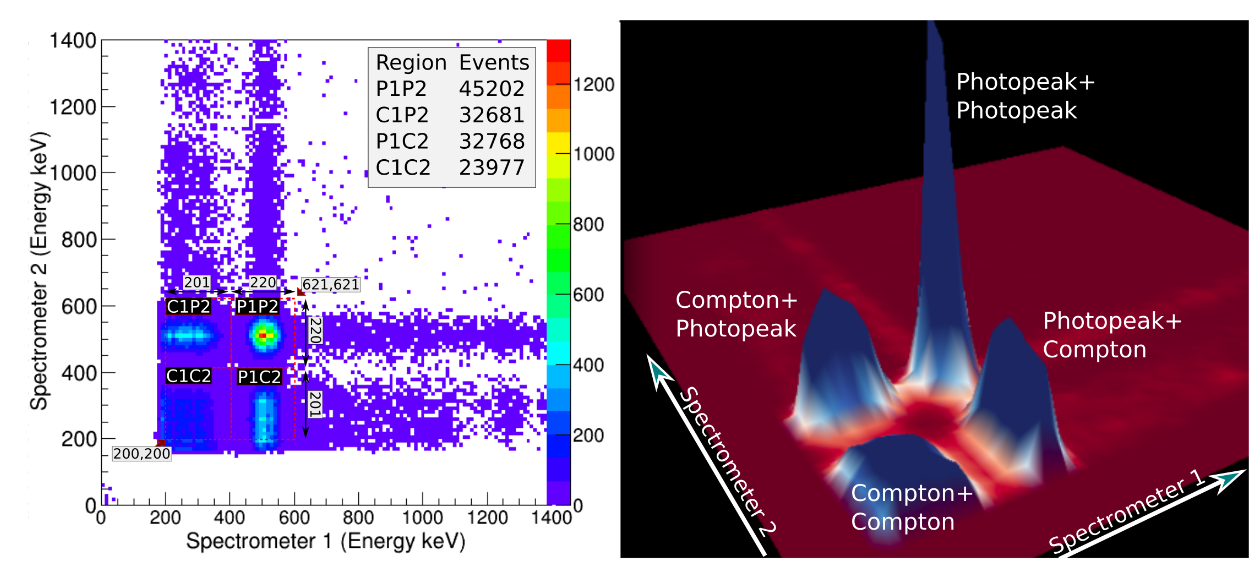
\includegraphics[width=1\columnwidth]{images/3d.png}
    \caption{The heat map and surface plot of the $^{22}$Na energy spectrum showing four significant peaks \cite{manual}}
    \label{3d}
\end{figure}

\section{Precautions}

    \begin{enumerate}
        \item The sample shouldn’t be touched, even though it’s
        in a case. After setting the appartus, it should not
        be disturbed.
        \item The histogram should be saved before starting the
        experiment.
        \item The coincidences should be measured in a longer
        time period, to increase the signal-to-noise ratio.
    \end{enumerate}

% \section{Conclusion}
